\chapter{Sistema de alimentación}

\section*{Resumen}

En este capítulo se presenta el diseño, dimensionamiento térmico, construcción y caracterización experimental del sistema de alimentación utilizado para los diferentes bloques del PLL.

\section{Introducción}

La alimentación constituye un aspecto fundamental en el diseño de un PLL, ya que las variaciones de tensión, el ruido y las perturbaciones presentes en las líneas de alimentación pueden afectar directamente el comportamiento de los bloques que conforman el sistema. En particular, el VCO presenta una elevada sensibilidad a las condiciones de polarización (\textit{pushing factor}), debido a que cualquier perturbación que modifique su punto de operación se traduce en una variación no deseada de la frecuencia de salida.

De manera similar, el filtro de lazo activo requiere una alimentación estable para garantizar que la tensión de control aplicada al VCO corresponda exactamente a la dinámica prevista durante el diseño. Variaciones o perturbaciones en su alimentación pueden introducir errores adicionales en dicha tensión de control y, en consecuencia, modificar el comportamiento dinámico del PLL.

Por este motivo, se diseñó una etapa de regulación independiente basada en un regulador lineal LM7805, cuya función es proporcionar una tensión regulada de $5~\mathrm{V}$ para la alimentación de los bloques correspondientes. Además del regulador, se incorporaron capacitores de desacoplo destinados a reducir las variaciones de tensión y las componentes de alta frecuencia presentes en la alimentación.

El sistema diseñado fue posteriormente evaluado mediante medición experimental, verificando que la tensión de salida se mantuviera en el valor nominal con bajo nivel de rizado.

\section{Diseño de la alimentación}

Para generar la tensión de alimentación requerida se seleccionó el regulador lineal LM7805. Este dispositivo permite obtener una tensión regulada nominal de $5~\mathrm{V}$ a partir de una tensión de entrada superior a dicho valor.

El circuito incorpora dos capacitores asociados al regulador. En la entrada se utiliza un capacitor de $0{,}33~\mu\mathrm{F}$, mientras que en la salida se incorpora un capacitor de $0{,}1~\mu\mathrm{F}$. Estos componentes contribuyen al desacoplamiento de la alimentación y a la estabilidad del regulador frente a variaciones de carga y perturbaciones de alta frecuencia.

El esquema implementado se muestra en la Figura~\ref{fig:alimentacion_esquema}.

\begin{figure}[H]
\centering
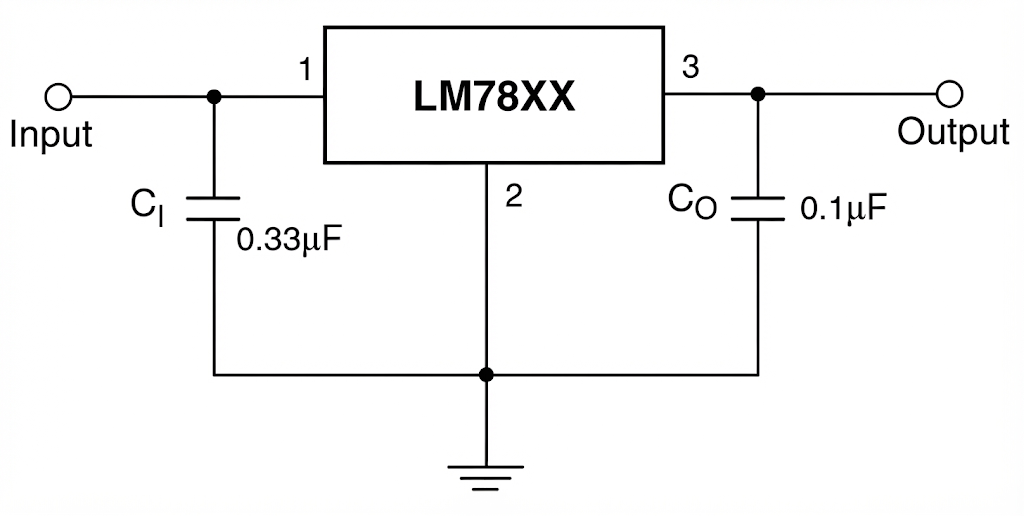
\includegraphics[width=0.65\textwidth]{imagenes/alimentacion_esquema.png}
\caption{Esquema de la etapa de alimentación basada en el regulador LM7805. (Fuente: \cite{LM7805}).}
\label{fig:alimentacion_esquema}
\end{figure}

\section{Cálculo de potencia disipada}
Para lograr independencia del generador de chirp con respecto a la conexión de red, se implementó la opción de conectar una batería de $9~\mathrm{V}$, regulando la tensión para obtener los $5~\mathrm{V}$ de salida. El consumo total medido del sistema es de $80~\mathrm{mA}$. La potencia disipada por el regulador se calcula como:

\begin{equation}
    P_D = (V_{\text{in}} - V_{\text{out}}) \cdot I_o
\end{equation}

\begin{equation}
    P_D = (9~\mathrm{V} - 5~\mathrm{V}) \cdot 0{,}08~\mathrm{A} = 0{,}32~\mathrm{W}.
\end{equation}

Para el encapsulado estándar TO-220, la resistencia térmica juntura-ambiente sin disipador ($\theta_{JA}$) es de aproximadamente $65~^\circ\mathrm{C/W}$ montado sobre una placa de circuito impreso. Suponiendo una temperatura ambiente máxima de trabajo de $T_A = 25~^\circ\mathrm{C}$, la elevación de temperatura y la temperatura de juntura resultan:

\begin{align}
    \Delta T &= P_D \cdot \theta_{JA} = 0{,}32~\mathrm{W} \cdot 65~^\circ\mathrm{C/W} = 20{,}8~^\circ\mathrm{C}, \\
    T_j &= T_A + P_D \cdot \theta_{JA} = 25~^\circ\mathrm{C} + 20{,}8~^\circ\mathrm{C} = 45{,}8~^\circ\mathrm{C}.
\end{align}

Dado que la temperatura máxima de juntura admisible especificada por el fabricante para el LM7805 \cite{LM7805} es de $125~^\circ\mathrm{C}$, el valor alcanzado de $45{,}8~^\circ\mathrm{C}$ se encuentra ampliamente por debajo del límite seguro. En consecuencia, el regulador opera en una zona segura de funcionamiento sin necesidad de incorporar un disipador de calor adicional.

\section{Desarrollo de la alimentación}

Para facilitar su utilización fuera del laboratorio, se desarrolló una etapa de alimentación con dos posibilidades de funcionamiento. El circuito permite alimentar el sistema mediante una fuente de continua externa o mediante una batería de $9~\mathrm{V}$. Esta configuración permite transportar el generador y realizar mediciones de campo sin depender de una conexión a la red eléctrica.

Los componentes utilizados en la implementación de la etapa de alimentación se detallan en la Tabla~\ref{tab:componentes_alimentacion}.

\begin{table}[H]
\centering
\begin{tabular}{|l|l|}
\hline
\textbf{Componente} & \textbf{Descripción} \\ \hline
Interruptor & Llave selectora de 3 posiciones \\ \hline
Batería & Batería alcalina de $9~\mathrm{V}$ \\ \hline
Placa & Placa experimental de pertinax/baquelita \\ \hline
Capacitor $C_{\text{out}}$ & $0{,}1~\mu\mathrm{F}$ cerámico \\ \hline
Capacitor $C_{\text{in}}$ & $0{,}33~\mu\mathrm{F}$ cerámico \\ \hline
Conector & Conector MTA para entrada de alimentación externa \\ \hline
Conector & Broche conector para batería de $9~\mathrm{V}$ \\ \hline
Regulador & LM7805 (encapsulado TO-220) \\ \hline
\end{tabular}
\caption{Componentes utilizados en la etapa de alimentación.}
\label{tab:componentes_alimentacion}
\end{table}

La Figura~\ref{fig:alimentacion_implementada} muestra la implementación física de la etapa de alimentación.

\begin{figure}[H]
\centering
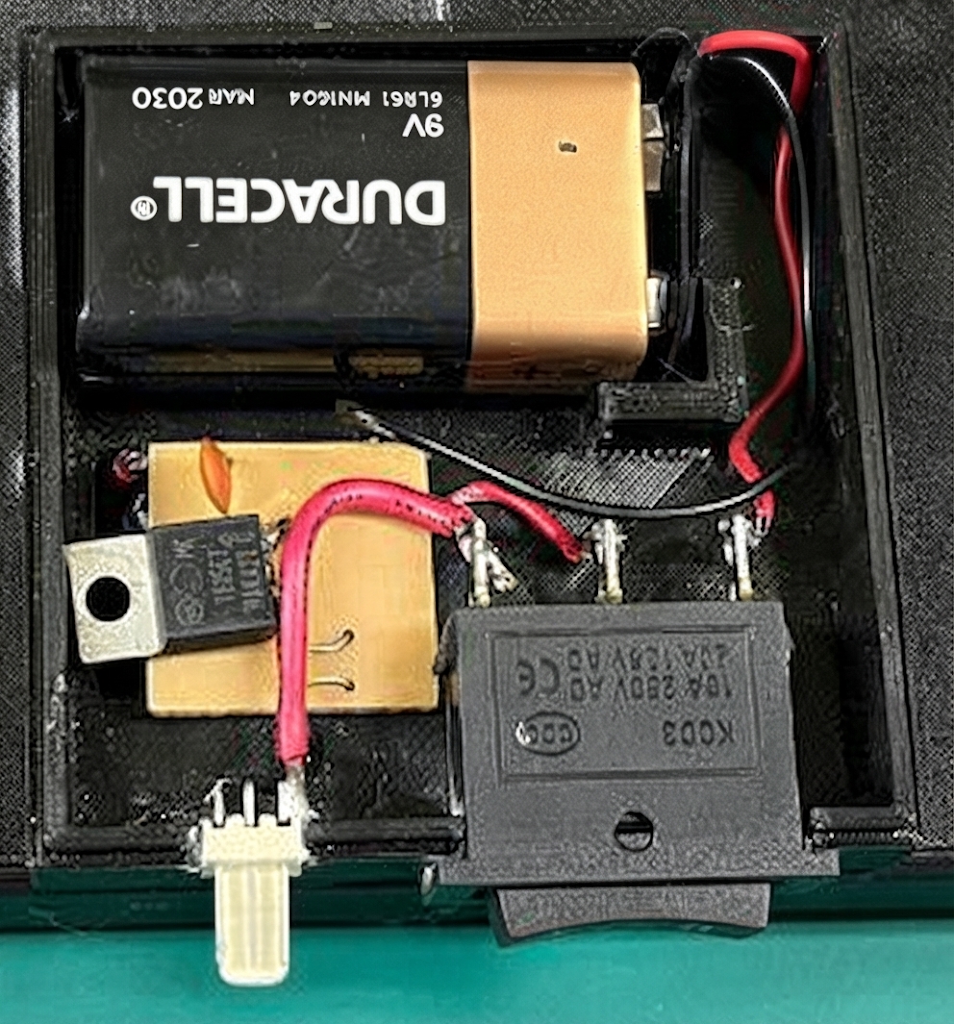
\includegraphics[width=0.35\textwidth]{imagenes/alimentacion_implementada.png}
\caption{Implementación física de la etapa de alimentación. (Fuente: Propia).}
\label{fig:alimentacion_implementada}
\end{figure}

\section{Medición}

Una vez implementada la etapa de alimentación, se realizó la medición experimental de la tensión continua y del rizado de salida con carga real conectada. Se obtuvo una tensión continua de salida de $5{,}11~\mathrm{V}$ y un rizado pico a pico de $5{,}8~\mathrm{mV}$, cuyas componentes de alta frecuencia son adicionalmente atenuadas por los capacitores de desacoplo locales de cada módulo.

La medición experimental se presenta en la Figura~\ref{fig:alimentacion_medicion}.

\begin{figure}[H]
    \centering
    \begin{subfigure}[b]{0.48\textwidth}
        \centering
        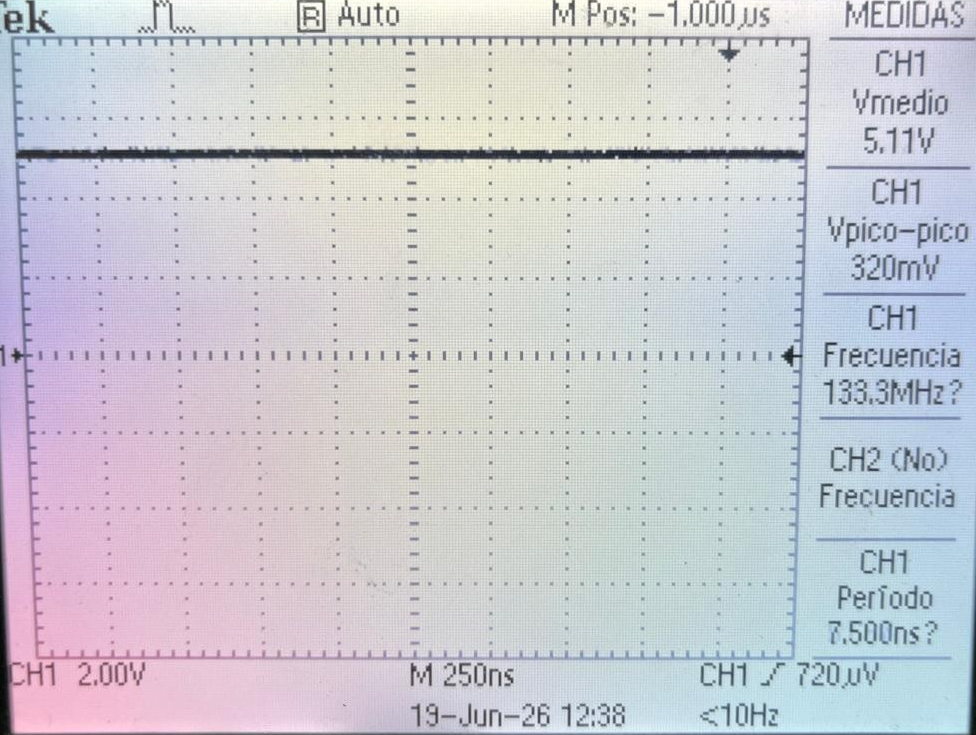
\includegraphics[width=\textwidth]{imagenes/tension_salida.png}
        \caption{Tensión continua de salida ($5{,}11~\mathrm{V}$).}
        \label{fig:tension_salida}
    \end{subfigure}
    \hfill
    \begin{subfigure}[b]{0.48\textwidth}
        \centering
        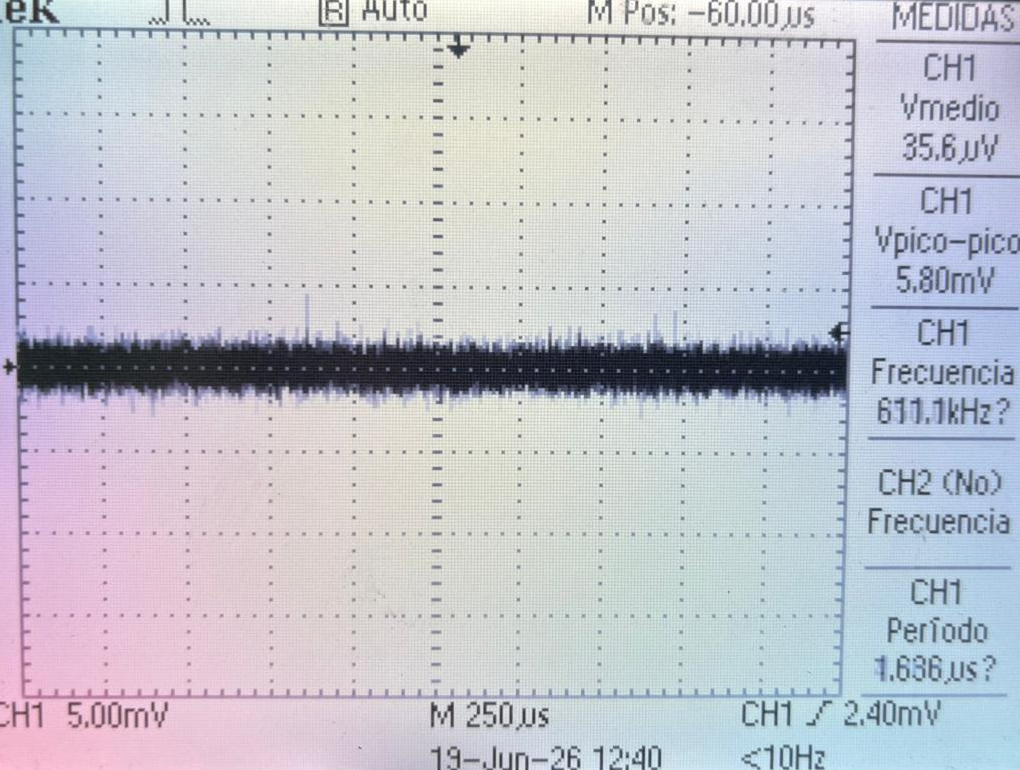
\includegraphics[width=\textwidth]{imagenes/riple.png}
        \caption{Rizado de la tensión de salida ($5{,}8~\mathrm{mV}$).}
        \label{fig:riple}
    \end{subfigure}
    \caption{Medición experimental de la etapa de alimentación. (Fuente: Propia).}
    \label{fig:alimentacion_medicion}
\end{figure}